\chapter{Introduzione}
\label{sec:intro}


\section[Background]{Background}

Sin dalla nascita delle prime \gls{CPU}, l'obiettivo principale degli ingegneri è stato quello di aumentare le prestazioni dei processori a livello hardware. Sono state sviluppate e applicate con successo diverse tecniche per aumentare le prestazioni, che includono l'uso di CPU pipelined per uamentare il throughput delle istruzioni, multilevel cache per nascondere la latenza di memoria e instruction level parallelism e processori superscalari per eseguire più istruzioni durante un ciclo di clock.
Quando ci si è accorti che queste metodologie non sarebbero bastate per tenere viva la legge di Moore \cite[]{Moore:law}, per aumentare ulteriormente le prestazioni si è passato a un approccio multi-core, che ha portato a una nuova forma di parallelismo, in cui alcune parti dell'applicazione possono essere eseguite in contemporanea su diversi core della stessa CPU. L'impatto delle CPU multi-core per accelerare le applicazioni è stato considerevole, ma il numero limitato di core che possono essere presenti sulla singola unità CPU è uno dei maggiori ostacoli che tutt'oggi limita l'incremento delle prestazioni. In fig. \ref{fig:moore_law} è mostrato come grazie alla tecnologia multi-core la legge di Moore è considerabile ancora valida.

\begin{figure}[ht]
\centering
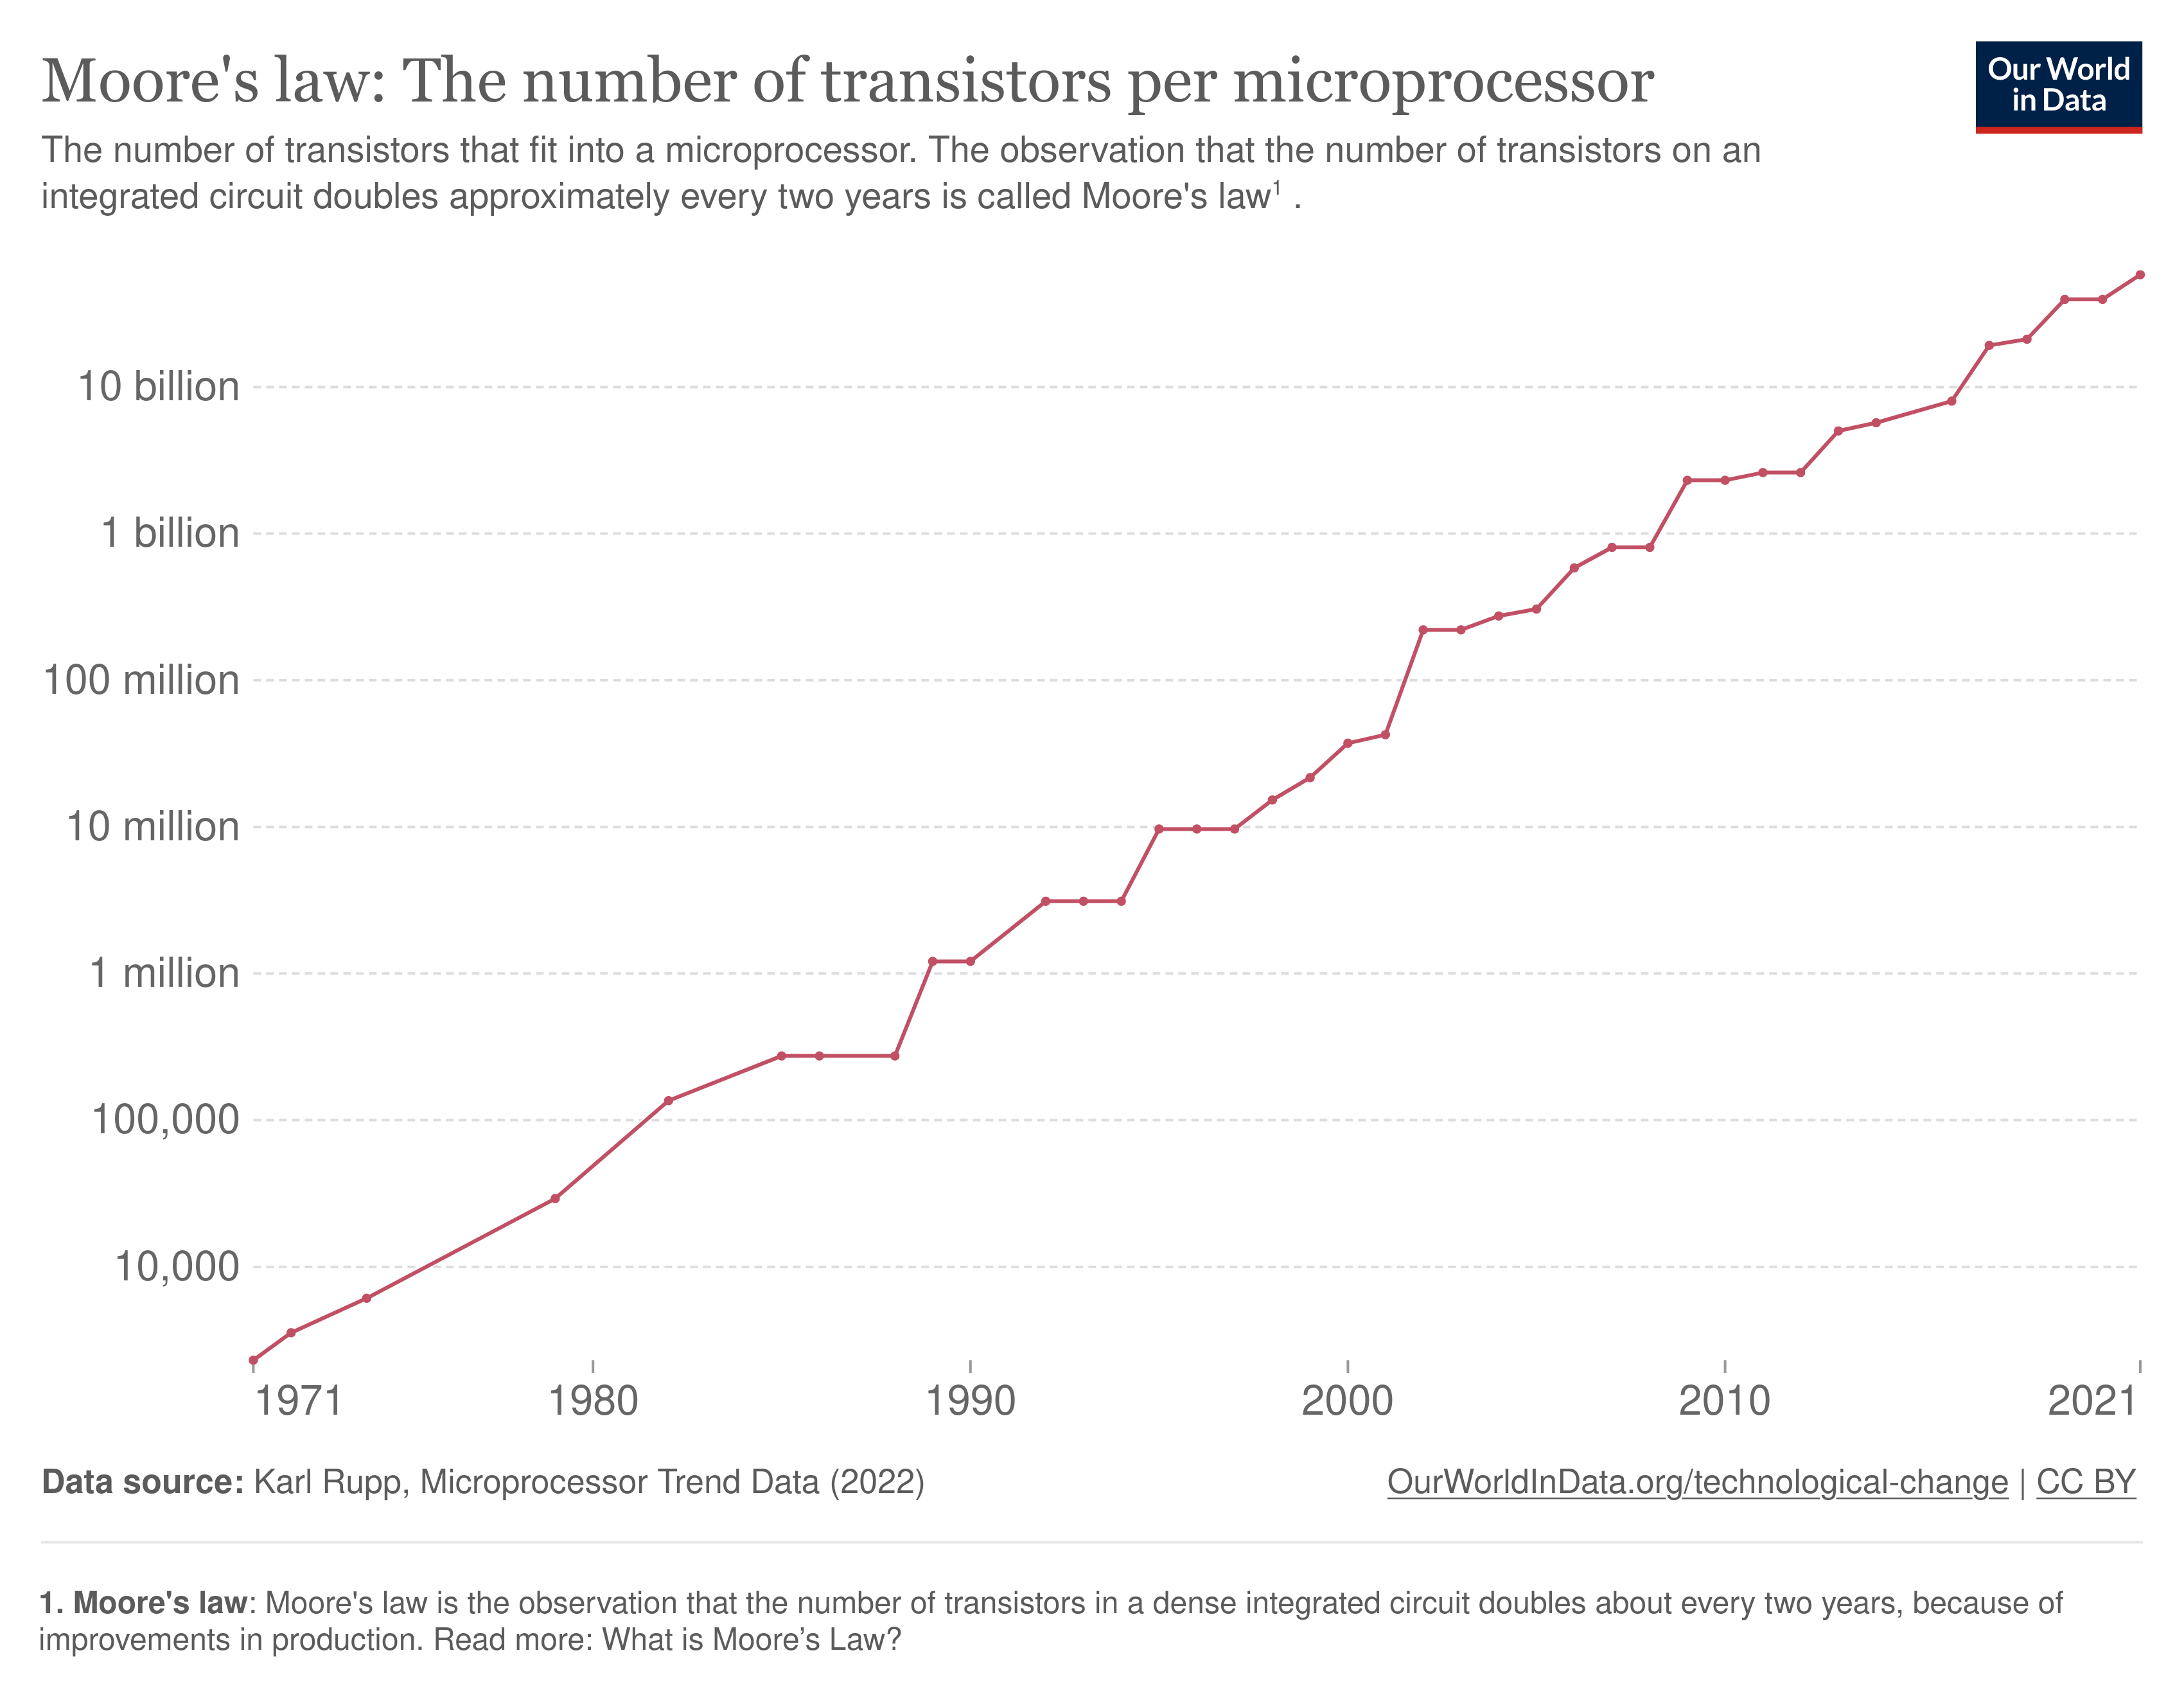
\includegraphics[width=.9\linewidth]{images/chapter1/moore_law2.png}
\caption{Legge di Moore}
\label{fig:moore_law}
\end{figure}

% GPU

Le \gls{GPU} sono hardware specializzato che prende a piene mani il concetto di multi-core e lo esalta, al punto da avere tantissimi core più semplici e lenti dei core di una CPU, ma con un più alto throughput totale. 
Originariamente sono state sviluppate per scopi legati all'elaborazione grafica, in particolare, per migliorare la resa delle immagini e la grafica 3D nei videogiochi, nelle applicazioni \gls{CAD} e nei software di modellazione e renderin. In seguito, le esigenze di una grafica sempre più dettagliata e complessa ha portato alla creazione di unità di elaborazione specializzate con un'architettura che le rende energicamente più efficienti di una CPU per algoritmi che processano grossi blocchi di dati in parallelo. Le GPU sono state quindi fruttate, anche per scopi diversi dall'elaborazione grafica e si sono rivelate particolamenti utili per applicazioni scientifiche, \gls{HPC} e tecniche che richiedono elaborazione intensive, come la simulazione, l'analisi dei dati e il calcolo scientifico. Adesso in particolare le GPU si sono particolarmente adatte per l'addestramento e l'implementazione di reti neurali, diventando uno strumento fondamentale per l'esplosione dell'intelligenza atrificiale e del machine learning.

% GPGPU

Quando si parla di \gls{GPGPU} si intende l'utilizzo delle GPU per compiti di calcolo generale, per renderle molto più che semplici dispositivi per l'elaborazione grafica. Questo è fondamentale per accelerare algoritmi di calcolo che richiedono enorme quantità di risorse, a patto che la computazione sia parallelizzabile su più processori.
Calcoli che prima richiedevano l'uso di supercomputer, per essere eseguiti, adesso si possono eseguire con una normale GPU desktop. 
Nel 2011 secondo la lista Top500, che classifica e descrive nel dettaglio i 500 sistemi informatici non distribuiti più potenti al mondo, il Tianhe-1A risultava il secondo supercomputer più potente al mondo, raggiungendo i 4.7 petaFLOPS di potenza computazionale, grazie a un sistema basasto sulle GPU Nvidia Tesla M2050 \cite[]{Tianhe-1A:link}. Solamente un anno dopo, invece, in in vetta alla classifica si trovò il Titan \cite[]{Titan:link} con un sistema basato sulle più recenti e performanti GPU Nvida Tesla K20X raggiungendo i 17.59 petaFLOPS di potenza.
Da quell'anno in poi divenne chiaro che le GPU erano diventate un componente essenziale nell'HPC tanto quanto lo erano nel desktop computing e dato che il supercomputing è il motore trainante di molte delle tecnologie che vediamo nei processori moderni, si è venuto a creare un circolo virtuoso per cui la necessità di processori sempre più veloci per elaborare dataset sempre più grandi, ha porta l'industria a produrre computer sempre più potenti. Ad oggi si sta delineando una divisione netta nella produzione di GPU per uso desktop e per uso scientifico, i principali produttori, quali AMD, Nvidia e, più recentemente, Intel, rilasciano prodotti ottimizzati per l'uno o per l'altro mercato, con lo scopo di soddisfare i requisiti richiesti da ogni settore. A giugno 2023 il supercomputer più veloce al mondo è il Frontier \cite[]{Frontier:link} con un sistema basato sulle GPU Radeon Instinct MI250X con coi riesce a raggiungere i 1.67 exaFLOPS, divenendo il primo exacale supercomputer al mondo. Grazie all'uso delle GPU in ambito HPC si sta riuscendo a incrementare le performance dei supercomputer in modo esponenziale, come si evince dalla fig. \ref{fig:supercomputer_flops}. L'incremento così repentino delle performance ha portato gli esperti di settore a scoprire una nuova legge empirica: la legge di Huang \cite[]{Huang:law}. Le performance delle GPU più che raddoppiano ogni due anni, in pratica, la legge di Huang è un'equivalente della legge di Moore, ma applicata alle GPU.

\begin{figure}[ht]
\centering
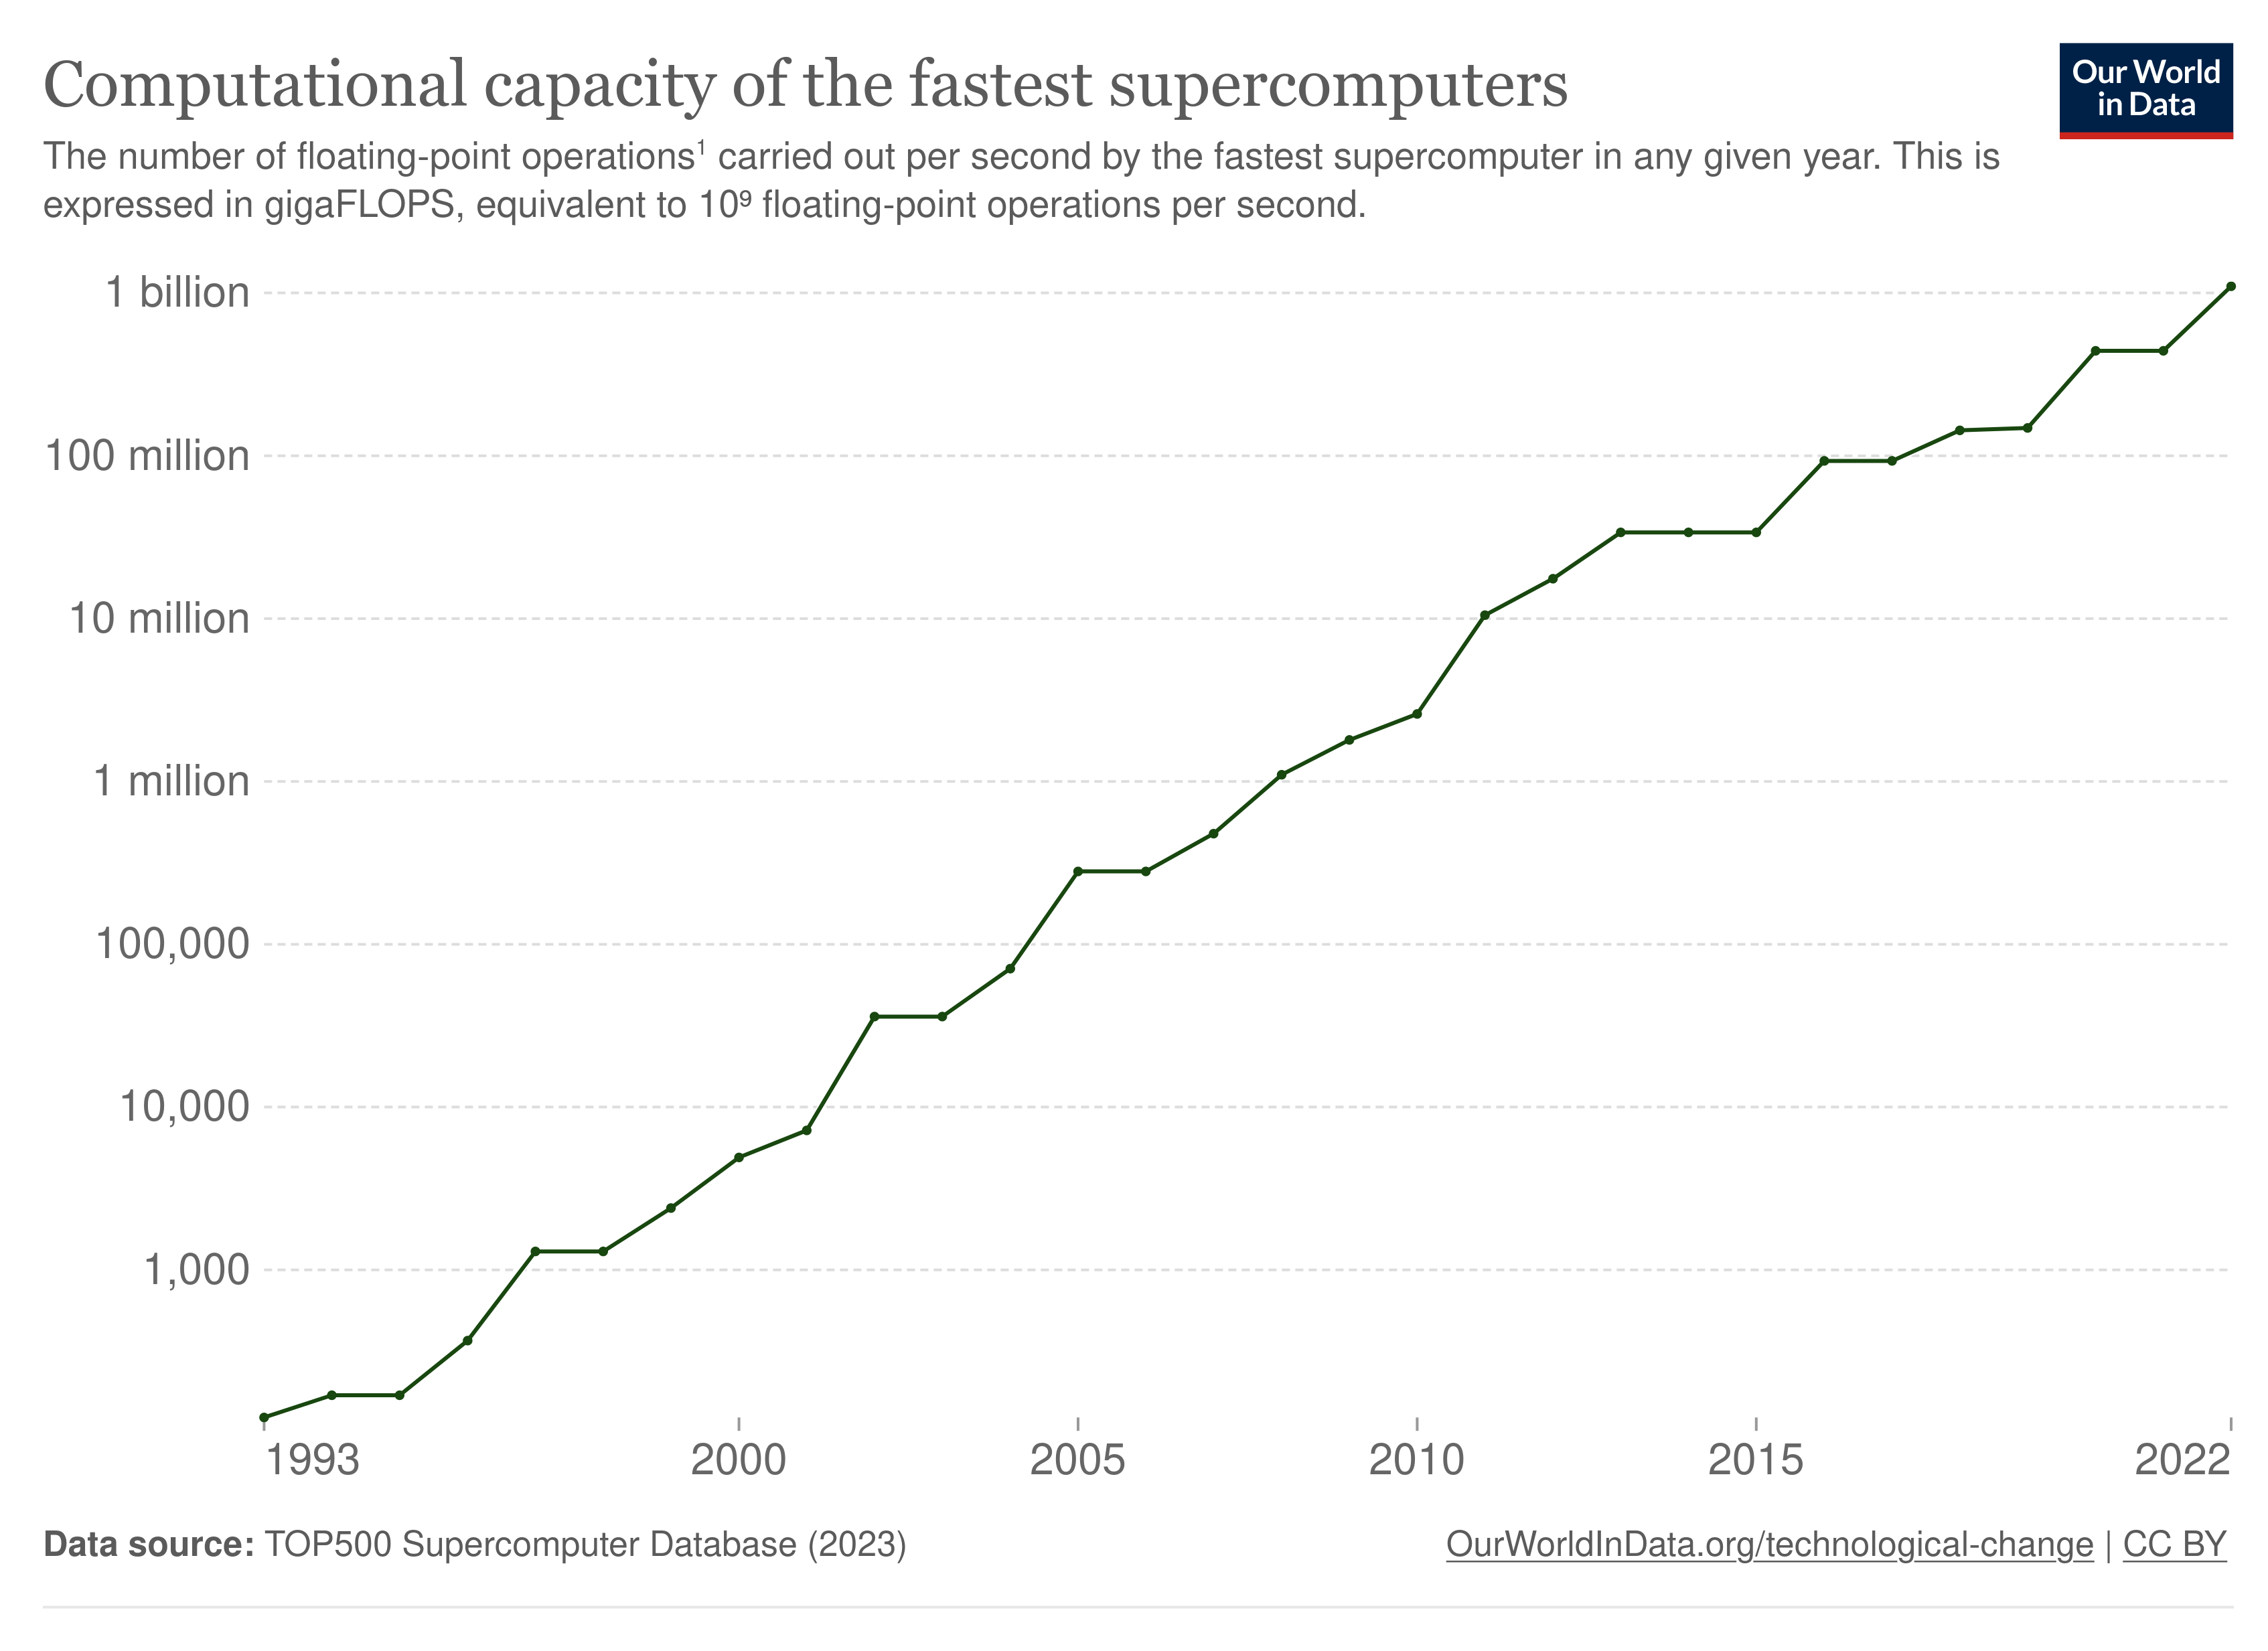
\includegraphics[width=.9\linewidth]{images/chapter1/supercomputer_flops.png}
\caption{Potenza dei supercomputer negli anni}
\label{fig:supercomputer_flops}
\end{figure}
    
%% Librerie GPU programming

Per poter programmare le GPU è risutanto necessario sviluppare delle \gls{API} che garantissero l'esecuzione del programma senza un'esplicita conversione dai dati in formato grafico. Le API oggi più utilizzate sono le \gls{CUDA} API di Nvidia \cite[]{Nvidia:CUDA} e le OpenCL API di Khronos Group \cite[]{KG:OpenCL}. Le API CUDA sfruttano l'omonima architettura delle GPU Nvidia e sono in formato proprietario, mentre le API OpenCL, come suggerisce il nome, sono uno standard aperto royalty-free e supportano la maggior parte delle archittetture GPU. Sebbene avesse prestazioni di molto inferiori rispetto a CUDA, OpenCL è storicamente stata la prima scelta per applicazioni multi-piattaforma, proprio per la sua natura open e la vasta quantità di hardware supportato. Nel 2015 Khronos Group annuncia le Vulkan API \cite[]{KG:Vulkan} e SPIR-V \cite[]{KG:SPIR-V}. Vulkan è una API grafica e di calcolo che offre un accesso ad alta efficienza e multi-piattaforma alle GPU moderne utilizzate in una vasta gamma di dispositivi, da PC e console ai telefoni cellulari e alle piattaforme embedded. Vulkan è stato progettato per sfruttare pesantemente il multithreading, permettendo la generazione di carichi di lavoro asincroni da parte di thread mulitpli della CPU che eseguono il codice sulla GPU solo dopo una esplicita sottomissione. Inoltre, la sua natura `close-to-metal' permette un controllo oculato delle risorse della GPU: lo sviluppatore è resposabile della sincronizzazione, allocazione di memoria e della sottomissione del lavoro, avendo così minor overhead del driver rispetto ad approcci come CUDA e OpenCL.

\begin{figure}[ht]
    \centering
    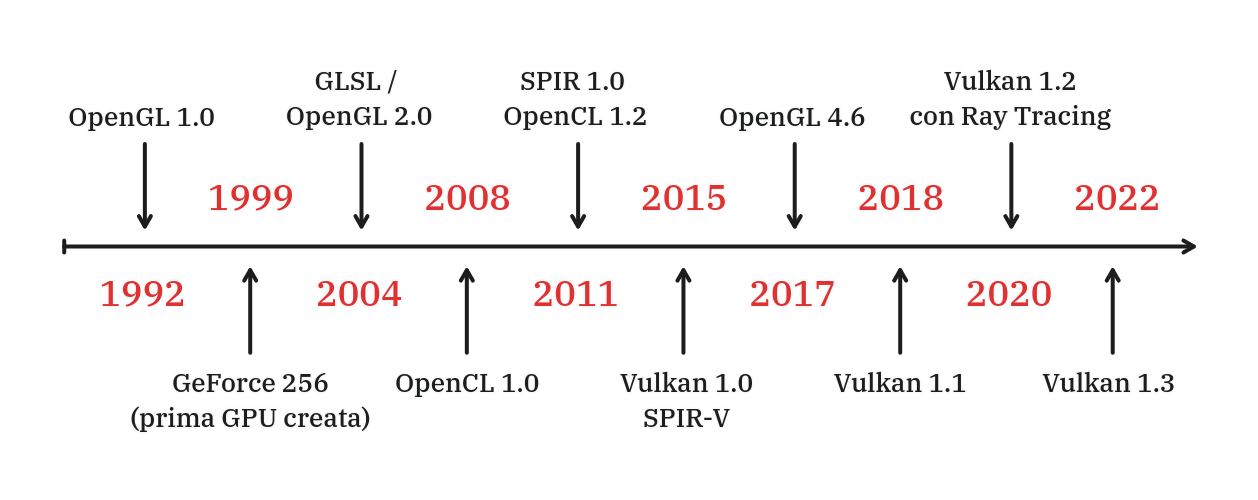
\includegraphics[width=.9\linewidth]{images/chapter1/vulkan_history.png}
    \caption{Contributi di Khronos Group nel tempo}
    \label{fig:vulkan_history}
\end{figure}

\section[Problema e Contributi]{Problema e Contributi}


L'elaborato si pone come obiettivo quello di trovare e valutare possibili vantaggi nello sviluppare un'applicazione di computing in Vulkan e Rust, per un ambiente a microservizi, rispetto a CUDA.
Nonostante Vulkan sia largamente usato nell'industria dei videogiochi, usarlo in ambito computing è una sfida non banale, a causa delle API verbose e del controllo meticoloso delle strutture dati. 
Un'idea per ridurre il carico intellettivo per lo sviluppatore, e rendere la develpement experience meno gravosa, può essere quella di consentire gestione della memoria in modo automatico, pur manetendo prestazioni quanto più vicine possibili a un'implementazione ``low level'', per questo motivo si è coniugato i vantaggi del linguaggio Rust con quelli che offre Vulkan. 

Per poter capire se Vulkan con Rust è una valida alternativa a CUDA per il computing bisogna rispondere alle seguenti domande:

% bullet points
\begin{itemize}
    \item Qual è il livello di performance che Vulkan riesce a raggiungere rispetto a CUDA? 
    \item Quanto è difficile sviluppare un'applicazione per il computing in Vulkan?
    \item In un ambiente a microservizi, quanto è facile sviluppare e mantenere un'applicazione Vulkan scritta in Rust? 
    \item Qual è il livello di maturità dell'ecosisistema Vulkan e quello di Rust?
\end{itemize}

Per rispondere a queste domande si è agito nel seguente modo:

\begin{itemize}
    \item Si è scelto di implementare algoritmi altamente parallelizzabili su GPU, quali la somma di vettori e moltiplicazione di matrici, da usare come banco di prova per comparare le performance di due medesime implementazioni in CUDA e Vulkan, in particolare è preso in considerazione sia il tempo dell'esecuzione ``pura'' dell'algoritmo, che del trasferimento dei dati dalla memoria host (CPU) a quella device (GPU).
    \item Si è implementato gli algoritmi in Vulkan per valutare il potenziale delle sue API close-to-metal e quanto ergonomico sia sviluppare mediante Rust. Dato che sviluppare in Vulkan richiede degli step standard quali la creazione di un logical device, una pipeline, la lettura del codice kernel e l'allocazione di memoria, si è usata la libreria Rust Vulkano \cite[]{github:Vulkano}, che implementa dei binding safe all'implementazione standard di Vulkan.
    \item Si è poi reimplementato i medesimi algoritmi in CUDA per comparare sia le performance che il diverso approccio alla scrittura dei kernel come estensione del linguaggio C++ tramite il compilatore nvcc \cite[]{Nvidia:nvcc}, osservando che GLSL \cite[]{KG:GLSL} usato in Vulkan offre più ottimizzazioni orientati alla grafica che al computing.
    \item Infine, considerando le necessità aziendali e i risultati relativi ai benchmark ottenuti, si è sviluppato un microservizio proof of concept che conuigare i vantaggi di Rust in ambito web e quelli di CUDA in ambito computing, valutando anche altri approcci nella soluzione del problema.
\end{itemize}



\section[Struttura della tesi]{Struttura della tesi}

!! TODO quando finiti tutti i capitoli

Il lavoro è stato progettato, sviluppato e testato con il supporto del team di Quantum Computing di Data Reply con sede a Torino. 

